\documentclass[12pt]{article}

\usepackage{graphicx}

\title{CS 372 Lab 4: IP}
\author{Ian Kronquist}

\begin{document}
\maketitle

\begin{enumerate}
    \item 192.168.43.114
        \begin{figure}[!ht]
            \centering
            \includegraphics[scale=0.5]{./p1.eps}
            \caption{First traceroute datagram}
        \end{figure}
    \item UDP (17)
    \item 20 bytes in the IP header. The payload for the IP header includes the UDP Data payload of 28 bytes + UDP header size of 5 bytes is 32 bytes.
    \item A datagram is fragmented if the fragment offset is greater than zero or the fragment bit is set. In this case, no flags are set.
    \item The identification always changes. As a result the header checksum also always changes. The identification must change to disambiguate possibly fragmented datagrams.
    \item The source and destination never change, otherwise the request would be lost or misdirected in transit.
    \item The identification values increase monotonically.
    \item The identification values include 0xeac7, 0xeac6, 0xeac5. The values of the TTL field include 64, 64, and 64.
    \item The first hop router is configured to use a sane TTL value, and since it is the first hop router the value is not decremented before it arrives at my host.
    \item Yes it has been fragmented.
        \begin{figure}[h]
            \centering
            \includegraphics[scale=0.5]{./p11.eps}
            \caption{First large fragmented traceroute datagram}
        \end{figure}

    \item The ``More Fragments'' bit in the flags field indicated that it has been fragmented. There are more fragments, in addition to that bit, I can also tell by looking at the fragment offsets of datagrams with the same identification.

        \begin{figure}[h]
            \centering
            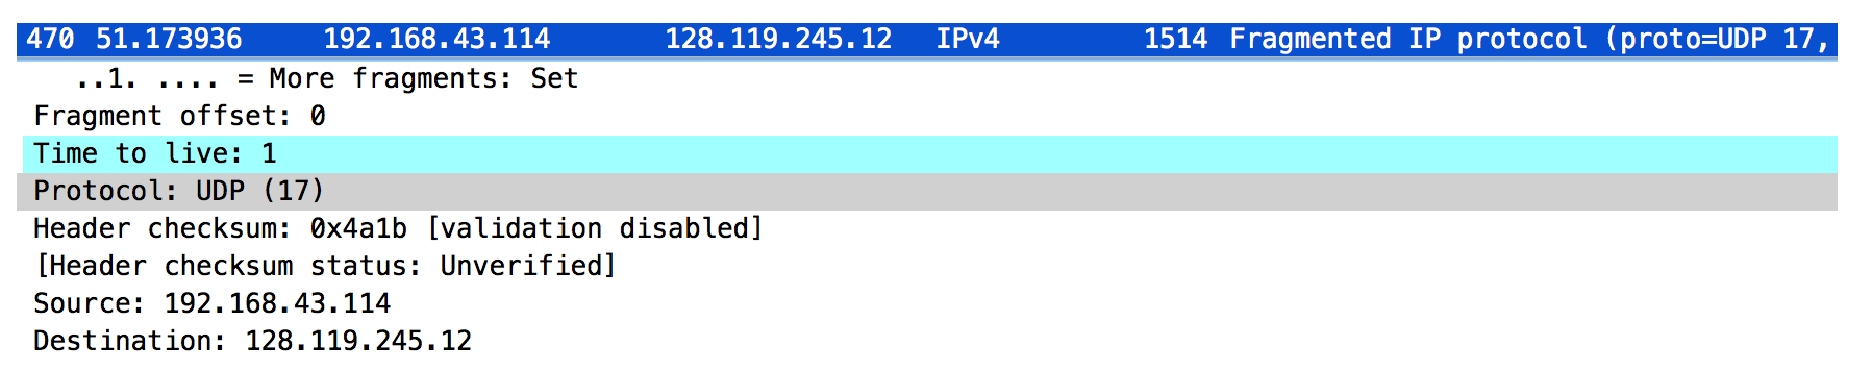
\includegraphics[scale=0.5]{./p12.eps}
            \caption{Second large fragmented traceroute datagram}
        \end{figure}



    \item The fragment offset is not zero which indicates that this is not the first fragment. The ``More Fragments'' bit is still set, so obviously there are more to come.
    \item Only the fragment offset and checksum change.

    \item Three fragments were created.
    \item The flags, checksums, and fragment offsets change.
\end{enumerate}

\end{document}
